\documentclass[a4paper]{article}

\usepackage[ngerman]{babel}
\usepackage[utf8]{inputenc}

\usepackage[scaled]{helvet}
\renewcommand{\familydefault}{\sfdefault}
\usepackage[T1]{fontenc}

\usepackage[margin=80pt]{geometry}

\usepackage{graphicx}
\usepackage{listings}
\usepackage{color}
\usepackage[table,xcdraw]{xcolor}
\usepackage [autostyle, german]{csquotes}
\MakeOuterQuote{"}

\definecolor{dkgreen}{rgb}{0,0.6,0}
\definecolor{gray}{rgb}{0.5,0.5,0.5}
\definecolor{mauve}{rgb}{0.58,0,0.82}

\lstset{frame=tb,
	language=Java,
	aboveskip=3mm,
	belowskip=3mm,
	showstringspaces=false,
	columns=flexible,
	basicstyle={\small\ttfamily},
	numbers=none,
	numberstyle=\tiny\color{gray},
	keywordstyle=\color{blue},
	commentstyle=\color{dkgreen},
	stringstyle=\color{mauve},
	breaklines=true,
	breakatwhitespace=true,
	tabsize=3
}


\title{\textbf{MOBPRO - Mobile Programming\\
Zusammenfassung FS 2019}}
\date{\today}
\author{Maurin D. Thalmann}

\begin{document}
	\pagenumbering{gobble}
	\maketitle
	\newpage
	\pagenumbering{arabic}
	\tableofcontents
	\newpage
	
	\section{Android 1 - Grundlagen}
	Apps sollen grundsätzlich gegen das aktuellste API entwickelt werden, aktuell API Level 28 Android 9 "Pie".
	Im Gradle-Build-Skript werden deshalb folgende SDK-Versionen festgehalten:
	\begin{description}
		\item[\textit{minSdkVersion}] Mindestanforderung an die SDK, Minimum-Version
		\item[\textit{targetSdkVersion}] Ziel-SDK-Version, auf welcher die App lauffähig sein soll
	\end{description}
	\textbf{ART (Android Runtime)} verwaltet Applikationen bzw. deren einzelne Komponenten:
	\begin{itemize}
		\item Komponente kann andere Komponente mit Intent-Mechanismus aufrufen
		\item Komponenten müssen beim System registriert werden (teilweise mit Rechten = Privileges)
		\item System verwaltet Lebenszyklus von Komponenten: Gestartet, Pausiert, Aktiv, Gestoppt, etc.
	\end{itemize}
\subsection{Komponenten}
	Applikationen sind aus Komponenten aufgebaut, die App verwendet dabei eigene Komponenten (min. eine) oder Komponenten von anderen, existierenden Applikationen.
\begin{table}[h!]
	\begin{tabular}{ll}
		\textbf{\textit{Name}}               & \textbf{\textit{Beschreibung}} \\
		\textbf{Activity}           & UI-Komponente, entspricht typischerweise einem Bildschirm \\
		\textbf{Service}            & Komponente ohne UI, Dienst läuft typischerweise im Hintergrund \\
		\textbf{Broadcast Receiver} & Event-Handler, welche auf App-interne oder \\ 
		   											& systemweite Broadcast-Nachrichten reagieren \\
		\textbf{Content Provider}   & Komponente, welche Datenaustausch zwischen versch. Applikationen ermöglicht
	\end{tabular}
\end{table}

\noindent
\textbf{Activity} entspricht einem Bildschirm, stellt UI-Widgets dar, reagiert auf Benutzer-Eingabe \& -Ereignisse. Eine App besteht meist aus mehreren Activities / Bildschirmen, die auf einem "Stack" liegen. \\
Basisklasse: \textit{android.app.Activity} \\
\textbf{Service} läuft typischerweise im Hintergrund für unbeschränkte Zeit, hat keine graphische Benutzer\-schnittstelle (UI), ein UI für ein Service wird immer von einer Activity dargestellt. \\
Basisklasse: \textit{android.app.Service} \\
\textbf{Broadcast Receiver} ist eine Komponente, welche Broadcast-Nachrichten empfängt und darauf reagiert. Viele Broadcasts stammen vom System (Neue Zeitzone, Akku fast leer,...), App kann aber auch interne Broadcasts versenden. \\
Basisklasse: \textit{android.content.BroadcastReceiver}\\
\textbf{Content Provider} ist die einzige \textit{direkte} Möglichkeit zum Datenaustausch zwischen Android-Apps. Bieten Standard-API für Suchen, Löschen, Aktualisieren und Einfügen von Daten. \\
Basisklasse: \textit{android.content.ContentProvider}
\subsection{Das Android-Manifest}
\textbf{AndroidManifest.xml} dient dazu, alle Komponenten einer Applikation dem System bekannt zu geben. Es enthält Informationen über Komponenten der Applikation, statische Rechte (Privileges), Liste mit Erlaubnissen (Permissions), ggf. Einschränkungen für Aufrufe (Intent-Filter). Es beschreibt die statischen Eigenschaften einer Applikation, beispielsweise: \\
\textit{(Diese Infos werden bei der App-Installation im System registriert, zusätzliche Infos (Version, ID, etc.) befinden sich im Gradle-Build-Skript (können build-abhängig sein))}

\begin{itemize}
	\item Java-Package-Name
	\item Benötigte Rechte (Internet, Kontakte, usw.)
	\item Deklaration der Komponenten
	\begin{itemize}
		\item Activities, Services, Broadcast Receivers, Content Providers
		\item Name (+ Basis-Package = Java Klasse)
		\item Anforderungen für Aufruf (Intent) für A, S, BR
		\item Format der gelieferten Daten für CP
	\end{itemize}
\end{itemize}
\newpage
\begin{figure}[htb!]
	\centering
	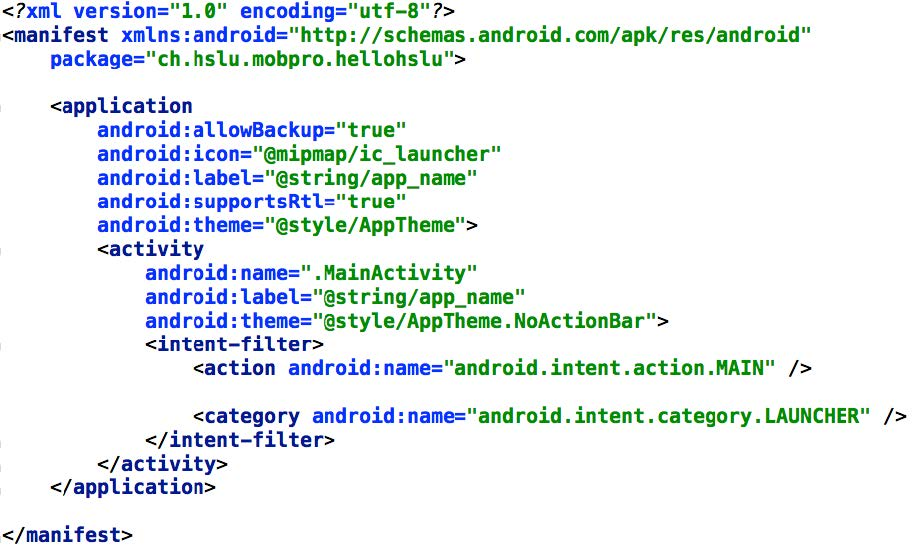
\includegraphics[width=12cm]{img/manifestxml.jpg}
	\caption{Beispiel eines Android-Manifests}
	\label{fig:manifestxml}
\end{figure}

	
	
	
	
\end{document}